%% =====================================================================
%%  Radiomics-based malignancy classification of pulmonary nodules
%%  IEEE journal format, TWO columns.  Compile:  latexmk -pdf main.tex
%%
%%  Red [TODO: ...] markers = things only the author can supply or decide.
%%  Search the file for \TODO to find them all.  Delete the macro's colour
%%  (see below) before submission.
%% =====================================================================
\documentclass[journal]{IEEEtran}

\usepackage[T1]{fontenc}
\usepackage[utf8]{inputenc}
\usepackage{amsmath,amssymb}
\usepackage{booktabs}
\usepackage{array}
\usepackage{graphicx}
\usepackage{xcolor}
\usepackage{tikz}
\usetikzlibrary{arrows.meta,positioning,fit,calc}
\usepackage{cite}
\usepackage[hidelinks]{hyperref}

% ---- helpers ---------------------------------------------------------
\newcommand{\TODO}[1]{\textcolor{red}{[TODO: #1]}}
\newcommand{\auc}{\mathrm{AUC}}
\newcommand{\ci}[2]{[#1,\,#2]}            % confidence interval  [lo, hi]
\newcommand{\code}[1]{\texttt{#1}}
\newcolumntype{R}{>{\raggedleft\arraybackslash}p{0.12\linewidth}}

\hyphenation{Py-Ra-di-o-mics ra-di-o-mics}
\setlength{\emergencystretch}{2.5em}

\begin{document}

\title{Radiomics for Pulmonary Nodule Malignancy on LUNA16/LIDC-IDRI:\\
A Leakage-Controlled and Fully Reproducible Evaluation}

\author{Lydia~Abraham%
\thanks{L. Abraham is with \TODO{affiliation, e-mail}.}%
\thanks{Code, tables and Docker image: \TODO{repository URL and commit hash}.}}

\markboth{Draft manuscript, \today}{Abraham: Radiomics for Pulmonary Nodule Malignancy}

\maketitle

\TODO{IMPORTANT: every number in Sections IV to VIII, the abstract and the tables was produced under the previous label (mean rating $\geq 3$). The label is now the dataset rule. Rerun the pipeline, then update all numbers from the new result files. Nothing below the label section is final.}

% =====================================================================
\begin{abstract}
This report documents an applied exercise in medical image data analysis: extracting handcrafted radiomic
features from pulmonary nodules and classifying radiologist-assessed malignancy with machine learning. From LUNA16/LIDC-IDRI we use 994 nodules from
551 patients that have both an image volume and a segmentation mask. For each nodule 107 PyRadiomics
features are extracted under two resampling protocols. The label is the mean radiologist rating
($\geq 3$ is malignant; 550 malignant, 444 benign). All comparisons are made with patient-grouped,
stratified cross-validation on 828 nodules, patient-level bootstrap confidence intervals, and a
sealed test set of 166 nodules (92 patients) that is scored once. Nodule diameter alone and scanner settings alone are used as simple reference models; they reach a
cross-validated $\auc$ of 0.828 and 0.530. Radiomics models score higher than the diameter reference
(by $+0.065$ $\auc$, 95\% CI $\ci{0.040}{0.091}$), with most of the difference coming from texture features. Six model families, tuned inside the training folds, differ by
less than 0.01 $\auc$, so the limit is set by the features and labels, not the learner. The selected
model (L2 logistic regression on diameter plus texture) reaches a test $\auc$ of 0.876
($\ci{0.812}{0.927}$) against 0.823 for diameter alone. A decision threshold chosen for 95\% recall on
cross-validated predictions gave a test sensitivity of 0.923 ($\ci{0.857}{0.976}$) at a specificity of
0.52, slightly below target. The complete pipeline, with unit tests and a Docker image, is released
to make every number reproducible.
\end{abstract}

\begin{IEEEkeywords}
Radiomics, pulmonary nodules, LIDC-IDRI, LUNA16, malignancy prediction, patient-level cross-validation,
data leakage, calibration, reproducibility.
\end{IEEEkeywords}

% =====================================================================
\section{Introduction}
\IEEEPARstart{R}{adiomics} converts medical images into large sets of quantitative features that
describe the shape, intensity and texture of a lesion~\cite{lambin2012radiomics,gillies2016radiomics}.
For pulmonary nodules, features of this kind are used to estimate how likely a nodule is to be
malignant. Reported results are often optimistic for reasons that have little to do with the images:
nodules of one patient appear on both sides of a train/test split, labels are derived from the same
ratings that are later used as inputs, tuning and evaluation share data, and the effect of nodule
size is never separated from the effect of texture~\cite{kapoor2023leakage,cawley2010overfitting,varma2006bias}.

The objective of this work is practical: to practise the full workflow of medical image data analysis on a
public dataset, that is, to prepare the data, extract radiomic features, train and evaluate classifiers, and
report the result honestly. We do not claim a new scientific finding. Where choices had to be made, such as
the label definition, the splitting scheme and the decision threshold, we describe them with their reasons, and we
take care to avoid the common evaluation errors listed above. Nodule diameter is included only as a simple reference
model against which the radiomics models are read; it is not a hypothesis under test.

\subsection*{Contributions}
\begin{enumerate}
  \item A leakage-controlled protocol: patient-level splits stratified by label and slice thickness,
        a single label column, rating-derived columns kept out of the modelling table, and a test set
        that is scored once (Sections~\ref{sec:data} and \ref{sec:design}).
  \item A comparison of the radiomics models with simple reference models (diameter, scanner settings), using
        confidence intervals on AUC differences and a check inside diameter strata
        (Section~\ref{sec:beyond}).
  \item A comparison of six tuned model families and an equal-weight ensemble, with tuning nested inside
        the training folds (Section~\ref{sec:models}).
  \item A recall-priority decision analysis with calibration, recall-target and cost-based thresholds,
        evaluated on the sealed test set (Sections~\ref{sec:threshold} and \ref{sec:test}).
  \item A complete, tested and containerised pipeline (Section~\ref{sec:repro}).
\end{enumerate}

% =====================================================================
\section{Related Work and Background}
\label{sec:related}
\textbf{Radiomics.} Radiomics pipelines extract hundreds of features per lesion from a segmented
volume~\cite{lambin2012radiomics,gillies2016radiomics}. PyRadiomics~\cite{vangriethuysen2017pyradiomics}
is the open-source extractor used here, and the Image Biomarker Standardization
Initiative~\cite{zwanenburg2020ibsi} defines reference values for most of its features.

\textbf{Data.} LIDC-IDRI~\cite{armato2011lidc} contains thoracic CT scans in which up to four
radiologists annotated nodules and rated their malignancy from 1 to 5. LUNA16~\cite{setio2017luna16}
is a curated subset of LIDC-IDRI built for nodule detection.

\textbf{Evaluation pitfalls.} Leakage between training and test data is a documented cause of
overstated results in machine-learning-based science~\cite{kapoor2023leakage}; using the same data for
model selection and performance estimation biases the estimate~\cite{cawley2010overfitting,varma2006bias};
and prediction-model reports should include calibration, not only
discrimination~\cite{steyerberg2010assessing}. We follow TRIPOD~\cite{collins2015tripod} and CLAIM~\cite{mongan2020claim}
reporting guidance (Section~\ref{sec:repro}).

\TODO{Add 3--5 papers on malignancy classification on LIDC-IDRI/LUNA16 (radiomics and deep learning) and
state, in one sentence each, how their evaluation protocol differs from this one. Do not compare
AUC values across papers unless the label definition and split are the same.}

% =====================================================================
\section{Data and Labels}
\label{sec:data}

\subsection{Dataset}
The metadata file lists one row per annotation (one radiologist's reading of one nodule). Volumes of
interest (VOIs) are CT crops around each nodule, supplied with binary nodule masks. After matching
annotations to files there are 994 VOI images and 996 masks; the 994 nodules with both an image and
a mask form the analysis set. They come from 551 patients; 234 patients contribute two or more
nodules, and these patients account for 68\% of all nodules. This clustering is why the unit of
splitting is the patient (Section~\ref{sec:design}).

Two data-handling decisions were needed:
\begin{itemize}
  \item \emph{Nodule identity.} Nodules are keyed by patient, nodule number and coordinates. Two distinct
        nodules of one patient (LIDC-IDRI-0332) share a nodule number; the single VOI file is assigned
        to the nodule whose coordinates lie closest to the VOI centre.
  \item \emph{Coordinate convention.} Metadata coordinates use the DICOM LPS convention. A check confirms
        that a VOI is an exact voxel crop of its CT scan, which validates the conversion.
\end{itemize}

We use the rule given by the dataset authors~\cite{setio2017luna16}: a nodule is malignant if \emph{at least two}
radiologists rated it above 3 (a 4 or a 5),
\begin{equation}
  y = \mathbb{1}\!\left[\, \sum_{i=1}^{n} \mathbb{1}[r_i > 3] \;\geq\; 2 \,\right],
  \label{eq:label}
\end{equation}
which gives 344 malignant (34.6\%) and 650 benign nodules. A first version of this work used a mean rating of at
least 3 instead; it was replaced because the dataset documentation defines the label by the rule above, and
using the documented rule keeps the results comparable with other work on this dataset. The rule is
count-based, so the same mean rating can map to different labels for nodules with different numbers of raters.
Nodules with exactly two ratings above 3 sit on the boundary of the rule, where a single different rating
would change the label. \TODO{Report how many of the 994 nodules this affects (the pipeline prints it) and
comment in your own words on what it means for label noise.}

Table~\ref{tab:labels} lists alternative definitions, used only for sensitivity analysis. The label threshold
(what \emph{malignant} means in the data) is a different decision from the decision threshold applied to model
probabilities (Section~\ref{sec:threshold}); only the latter is tuned.

\begin{table}[!t]
\caption{Label definitions considered. Counts are for the 994 analysis nodules.}
\label{tab:labels}
\centering\small
\begin{tabular}{lrr}
\toprule
Definition & Malignant & Benign\\
\midrule
Mean rating $> 3$                         & 404 & 590\\
Mean rating $\geq 3$                      & 550 & 444\\
Mean rating $\geq 2.7$                    & 634 & 360\\
Mean rating $\geq 2.5$                    & 770 & 224\\
\textbf{At least two ratings of 4 or 5 (used)} & \textbf{344} & \textbf{650}\\
\bottomrule
\end{tabular}
\end{table}

\textbf{The label definition changes the size baseline substantially.}
Table~\ref{tab:labelsens} gives the cross-validated $\auc$ of diameter alone under each definition (trainval,
the locked folds). It ranges from 0.746 to 0.923. Counting ties as malignant makes the task harder than treating
them as benign (0.828 vs 0.884) or removing them (0.900), because nodules at exactly 3.0 are by construction the
most ambiguous. Every comparison with the diameter reference is therefore conditional on the label, and
the difference reported here ($+0.065$) is not a property of the images alone.
\TODO{Rerun the primary comparison (diameter vs \code{diameter\_texture} vs \code{radiomics}) under at least the
``ties benign'', ``ties excluded'' and ``dataset rule'' labels and add the paired differences here.}

\begin{table}[!t]
\caption{Diameter-only cross-validated $\auc$ under alternative label definitions (trainval, $n=828$ unless stated).}
\label{tab:labelsens}
\centering\small
\resizebox{\columnwidth}{!}{\begin{tabular}{lrc}
\toprule
Label definition & Malignant & Diameter-only $\auc$\\
\midrule
At least two ratings of 4 or 5 (dataset rule) & 292 & 0.923\\
Ties excluded (mean $>3$ vs $<3$; $n=703$)    & 334 & 0.900\\
Mean rating $>3$ (ties benign)                & 334 & 0.884\\
\textbf{Mean rating $\geq3$ (used)}           & \textbf{459} & \textbf{0.828}\\
Mean rating $\geq 2.7$                        & 529 & 0.813\\
Mean rating $\geq 2.5$                        & 642 & 0.746\\
\bottomrule
\end{tabular}}
\end{table}

\subsection{Leakage controls}
\begin{itemize}
  \item \textbf{One label column.} The modelling table contains the binary label only. Ratings, their mean,
        the number of raters and the tie flag are stored in a separate audit file, because a column such as
        the mean rating is the label before thresholding.
  \item \textbf{No extent features.} Image-extent and bounding-box columns of the VOI are not used as inputs,
        because they are proxies for nodule size that bypass the radiomics.
  \item \textbf{Patient-level grouping.} A model that sees only scanner settings (in-plane pixel size and slice
        thickness) reaches $\auc=0.60$ under a random nodule-level split but 0.54 under a patient-grouped split.
        The difference is patient information leaking across the split.
\end{itemize}

% =====================================================================
\section{Feature Extraction}
\label{sec:features}
Features are extracted with PyRadiomics 3.0.1~\cite{vangriethuysen2017pyradiomics} from each VOI and mask
(3-D, label 1, no image filters, intensities in Hounsfield units, discretised with a fixed bin width of 25).
Image and mask geometry (size, spacing, origin, direction) must match exactly or the nodule is rejected.
Each nodule yields 107 features (Table~\ref{tab:features}; the full list is in Appendix~\ref{app:features}),
under two protocols:
\begin{description}
  \item[\code{original\_spacing}:] the image is used as recorded; voxel size differs between patients.
  \item[\code{isotropic\_1mm}:] image resampled to $1\times1\times1$\,mm voxels by B-spline interpolation
        (masks by nearest neighbour) before extraction.
\end{description}
Extraction depends only on image and mask, never on labels or splits, so changing the label or the split
never requires re-extraction. The run produced $994\times 2 = 1988$ feature rows with no failures
and takes a few minutes on a laptop CPU.

\begin{table*}[!t]
\caption{PyRadiomics feature classes used (107 features).}
\label{tab:features}
\centering\small
\begin{tabular}{lrp{0.62\linewidth}}
\toprule
Class & $n$ & What it describes\\
\midrule
Shape (3-D)     & 14 & Volume, surface area, diameters, axis lengths, sphericity, elongation, flatness\\
First order     & 18 & Distribution of voxel intensities (mean, spread, skewness, entropy, energy)\\
GLCM            & 24 & Co-occurrence of intensities in neighbouring voxels (contrast, correlation, homogeneity)\\
GLRLM           & 16 & Runs of equal intensity (short vs long runs)\\
GLSZM           & 16 & Connected zones of equal intensity (small vs large zones)\\
GLDM            & 14 & Dependence of a voxel on similar neighbours\\
NGTDM           &  5 & Difference between a voxel and its neighbourhood (coarseness, busyness)\\
\midrule
Total           & 107 & Texture $=$ GLCM$+$GLRLM$+$GLSZM$+$GLDM$+$NGTDM $=75$\\
\bottomrule
\end{tabular}
\end{table*}

\TODO{Add the result of the mask-resampling robustness check (pipeline stage 5): how many features keep
their rank when the mask is resampled, and what you conclude.}

% =====================================================================
\section{Experimental Design}
\label{sec:design}

\subsection{Overview}
Figure~\ref{fig:pipeline} shows the ten pipeline stages. Stages 1--9 use only the 828 trainval nodules;
the sealed test set is touched once, by stage 10.

\begin{figure*}[!t]
\centering
\resizebox{0.95\textwidth}{!}{%
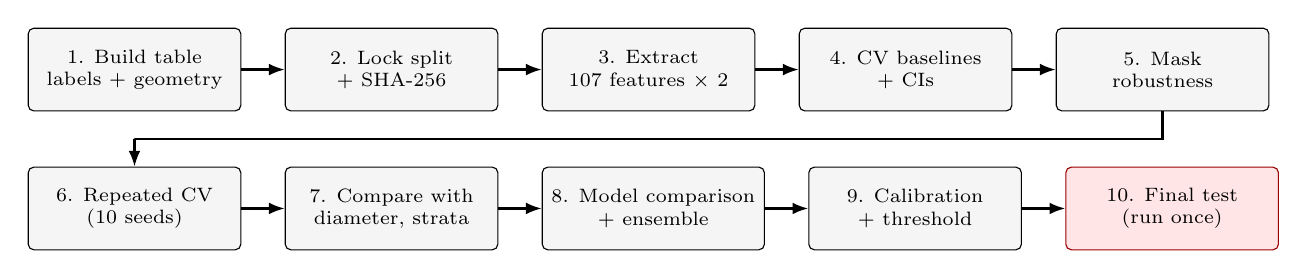
\begin{tikzpicture}[
  box/.style={draw, rounded corners=2pt, align=center, minimum width=2.7cm, minimum height=1.05cm, font=\scriptsize, fill=gray!8},
  sealed/.style={box, fill=red!10, draw=red!60!black},
  arr/.style={-{Latex[length=2mm]}, thick}]
  \node[box] (s1) {1. Build table\\labels + geometry};
  \node[box, right=0.55cm of s1] (s2) {2. Lock split\\+ SHA-256};
  \node[box, right=0.55cm of s2] (s3) {3. Extract\\107 features $\times$ 2};
  \node[box, right=0.55cm of s3] (s4) {4. CV baselines\\+ CIs};
  \node[box, right=0.55cm of s4] (s5) {5. Mask\\robustness};
  \node[box, below=0.7cm of s1] (s6) {6. Repeated CV\\(10 seeds)};
  \node[box, right=0.55cm of s6] (s7) {7. Compare with\\diameter, strata};
  \node[box, right=0.55cm of s7] (s8) {8. Model comparison\\+ ensemble};
  \node[box, right=0.55cm of s8] (s9) {9. Calibration\\+ threshold};
  \node[sealed, right=0.55cm of s9] (s10) {10. Final test\\(run once)};
  \draw[arr] (s1)--(s2); \draw[arr] (s2)--(s3); \draw[arr] (s3)--(s4); \draw[arr] (s4)--(s5);
  \draw[arr] (s5.south) -- ++(0,-0.35) -| ($(s6.north)+(0,0.35)$) -- (s6.north);
  \draw[arr] (s6)--(s7); \draw[arr] (s7)--(s8); \draw[arr] (s8)--(s9); \draw[arr] (s9)--(s10);
\end{tikzpicture}}
\caption{Pipeline. Each stage reads files written by earlier stages and writes its own tables. Stages 1--9 use
cross-validation on trainval only; stage 10 (red) scores the sealed test set once.}
\label{fig:pipeline}
\end{figure*}

\subsection{Patient-level split}
\label{sec:split}
A stratified, grouped $K$-fold splitter~\cite{pedregosa2011sklearn} with seed 42 and groups equal to the patient
identifier cuts the data into six chunks of about 166 nodules. One chunk is the \emph{sealed test set}
(166 nodules, 92 patients, 91 malignant); the other five are the cross-validation folds on the remaining
828 trainval nodules. No patient appears in more than one chunk. The strata are the label combined with
slice-thickness group (thin $\leq1.0$\,mm, 1.25\,mm, thick $\geq1.8$\,mm), so that both malignancy and
the dominant acquisition difference are balanced across chunks. The split file is written once and locked
with its SHA-256 hash (recorded in the decision log), and every later stage validates it before use.

Stratification matters. Averaged over 20 seeds, the standard deviation of the malignant share across
folds is 0.004 with stratification and 0.042 with grouping alone, and the spread in fold size is 1.4
versus 29.7 nodules. Table~\ref{tab:folds} shows the folds that were used. A diameter-only probe over
20 seeds shows that the cross-validation estimate is stable (mean $\auc$ 0.828, std 0.006) whereas the
single-chunk test estimate is not (mean 0.827, std 0.028, range 0.774--0.878). Hence (i) the test set is
fixed once and never re-drawn, (ii) the test result is reported with a confidence interval, and
(iii) model comparison relies on cross-validation.

\begin{table*}[!t]
\caption{Chunks of the locked split (seed 42).}
\label{tab:folds}
\centering\small
\begin{tabular}{lrrrrr}
\toprule
Chunk & Nodules & Patients & Malignant share & Mean diam.\ (mm) & Thick-slice share\\
\midrule
Test    & 166 & 92 & 0.548 & 8.45 & 0.386\\
Fold 0  & 166 & 92 & 0.554 & 8.31 & 0.386\\
Fold 1  & 166 & 92 & 0.554 & 8.59 & 0.380\\
Fold 2  & 165 & 90 & 0.552 & 9.13 & 0.388\\
Fold 3  & 165 & 92 & 0.558 & 8.76 & 0.388\\
Fold 4  & 166 & 93 & 0.554 & 8.91 & 0.386\\
\bottomrule
\end{tabular}
\end{table*}

\subsection{Input sets}
Models are trained on named input sets (Table~\ref{tab:inputs}). The size and scanner baselines
are the yardsticks against which radiomics are judged.

\begin{table}[!t]
\caption{Input sets.}
\label{tab:inputs}
\centering\small
\resizebox{\columnwidth}{!}{\begin{tabular}{llr}
\toprule
Name & Contents & Features\\
\midrule
\code{diameter}             & nodule diameter (mm, from metadata) & 1\\
\code{scanner}              & in-plane pixel size, slice thickness & 2\\
\code{shape\_only}          & PyRadiomics shape features & 14\\
\code{firstorder\_only}     & first-order features & 18\\
\code{texture\_only}        & GLCM, GLRLM, GLSZM, GLDM, NGTDM & 75\\
\code{radiomics\_no\_shape} & first order $+$ texture & 93\\
\code{radiomics}            & all PyRadiomics features & 107\\
\code{combined}             & diameter $+$ \code{radiomics} & 108\\
\code{diameter\_texture}    & diameter $+$ texture & 76\\
\code{diameter\_firstorder} & diameter $+$ first-order & 19\\
\bottomrule
\end{tabular}}
\end{table}

\subsection{Models}
\label{sec:modelsdef}
All models start with median imputation (and standardisation where applicable) fitted on the training fold
only. Table~\ref{tab:grids} lists the families and the (deliberately small) hyper-parameter grids; 828
nodules cannot support a large search. Hyper-parameters are chosen \emph{inside} each training fold by
3-fold patient-grouped cross-validation maximising AUC, so the validation fold never influences tuning.
\texttt{logreg} is the untuned reference ($C=1$). The ensemble is the equal-weight average of the predicted
probabilities of L2 logistic regression, random forest and gradient boosting; it has no fitted weights and
therefore cannot leak. Stacking was not used: it learns weights from strongly correlated base models on a
small sample and needs a nested patient-grouped scheme to be valid.

\begin{table*}[!t]
\caption{Model families and tuning grids (tuned inside each training fold).}
\label{tab:grids}
\centering\small
\begin{tabular}{p{0.20\linewidth}p{0.20\linewidth}p{0.48\linewidth}}
\toprule
Model & Family & Grid\\
\midrule
\code{logreg}        & linear & none ($C=1$)\\
\code{logreg\_l2}    & linear & $C\in\{0.001,0.01,0.1,1\}$\\
\code{logreg\_enet}  & linear~\cite{zou2005elasticnet} & $C\in\{0.01,0.1,1\}$, L1 share $\in\{0.2,0.5,0.8\}$\\
\code{random\_forest}& trees~\cite{breiman2001rf} & 300 trees; min.\ leaf $\in\{1,3,8\}$; features per split $\in\{\sqrt{p},0.3p\}$\\
\code{hist\_gb}      & boosting~\cite{friedman2001gbm} & 200 iterations; learning rate $\in\{0.03,0.1\}$; leaves $\in\{4,8\}$; L2 $\in\{0,1\}$\\
\code{svm\_rbf}      & kernel & $C\in\{0.3,1,3,10\}$, $\gamma\in\{\text{scale},0.003\}$\\
\code{ensemble\_avg} & average & mean of \code{logreg\_l2}, \code{random\_forest}, \code{hist\_gb}\\
\bottomrule
\end{tabular}
\end{table*}

\subsection{Prior exploratory work and independence of the test set}
\label{sec:disclosure}
An earlier exploratory analysis of this dataset by a collaborator used the dataset's own label rule (at least two
ratings above 3) and the same seed. Because the split is stratified by label, the present split differs from it. The earlier
analysis scored its own test chunk (166 nodules, 91 patients) once, as a baseline, and those results were not used for any
choice made here. The present test chunk overlaps with that earlier test chunk by 22 nodules (13\%) and 12 patients (13\%);
the other 87\% of present test patients were part of the earlier training and validation data, on which feature-stability
and resampling analyses had been run, and which may have informed the choice of feature classes, bin width and protocols.
All model, input, protocol and threshold choices in this work were made from cross-validation on the present trainval
nodules. The test set is therefore sealed with respect to the present analysis, but not untouched by the project as a whole.

\subsection{Metrics and uncertainty}
We report the area under the ROC curve ($\auc$) and average precision (AP) for discrimination, the Brier
score, calibration intercept and slope~\cite{steyerberg2010assessing} for calibration, and sensitivity,
specificity, positive and negative predictive value at a threshold. Three kinds of uncertainty are kept separate:
\begin{enumerate}
  \item \emph{Patient sampling.} 95\% percentile intervals from 2000 bootstrap replicates that resample
        \emph{patients}, not nodules~\cite{efron1993bootstrap}; resampling nodules would understate the
        interval because nodules of a patient are correlated.
  \item \emph{Fold assignment.} Cross-validation repeated under 10 different fold assignments (seeds 42--51);
        we report the mean and range of $\auc$.
  \item \emph{Paired differences.} For a comparison of two models the bootstrap evaluates both on the
        identical resample and reports the interval of $\auc_A-\auc_B$. Looking at whether two separate
        intervals overlap is not a valid comparison.
\end{enumerate}
Eleven or more comparisons are made in some sections and no multiplicity correction is applied; borderline
intervals are therefore described as suggestive rather than as findings.

\subsection{Decision threshold}
Let $\hat p$ be the predicted probability. A nodule is flagged when $\hat p\geq t$. Two ways of choosing $t$
are studied, both from out-of-fold predictions on trainval only:
\begin{itemize}
  \item \textbf{Recall target.} $t$ is the largest value for which cross-validated sensitivity is at least a target
        (90\%, 95\% or 98\%).
  \item \textbf{Cost ratio.} If a missed malignancy is $k$ times as costly as a false alarm, the cost-minimising
        cutoff of a calibrated model is $t=1/(1+k)$.
\end{itemize}
Equivalently, a cutoff $t$ implies $k=(1-t)/t$. The recall-95\% rule was fixed before the test set was scored.

\subsection{Pre-declared test protocol}
Before the test set was scored, the following were written in the decision log (Appendix~\ref{app:decisions}):
the protocol, the primary and secondary model with their inputs, the two thresholds, and the statement that
no other model would be scored. A diameter-only logistic regression is scored as a reference for context; it
is not a candidate. The scoring script refuses to run without explicit confirmation, refuses if the thresholds
differ from those produced in cross-validation, refuses if the split file hash differs, and refuses a second run.

% =====================================================================
\section{Results}
\label{sec:results}

\subsection{What the feature families can do}
\label{sec:baselines}
Table~\ref{tab:baselines} gives the cross-validated results of logistic regression ($C=1$) on each input set,
averaged over 10 fold assignments, for both protocols. Scanner settings alone are at chance, so the features
are not simply detecting the scanner. Diameter alone is already strong ($\auc=0.828$): size is the baseline that
radiomics must beat. Adding shape, first-order and texture features raises $\auc$ monotonically up to 0.894 with
original spacing, and texture is the most informative family.

\begin{table*}[!t]
\caption{Cross-validated $\auc$ (10 repeats; mean, range over repeats, 95\% patient-bootstrap CI), logistic regression
($C=1$), trainval, $n=828$.}
\label{tab:baselines}
\centering\small
\begin{tabular}{lccc}
\toprule
 & Mean (range) & 95\% CI & Mean, 1\,mm isotropic\\
Input &  \multicolumn{2}{c}{original spacing} & (95\% CI)\\
\midrule
\code{diameter}            & 0.828 (0.825--0.830) & $\ci{0.799}{0.857}$ & 0.828 ($\ci{0.799}{0.857}$)\\
\code{scanner}             & 0.530 (0.501--0.541) & $\ci{0.483}{0.578}$ & 0.530 ($\ci{0.483}{0.578}$)\\
\code{shape\_only}         & 0.852 (0.849--0.854) & $\ci{0.825}{0.878}$ & 0.847 ($\ci{0.820}{0.874}$)\\
\code{firstorder\_only}    & 0.865 (0.862--0.869) & $\ci{0.838}{0.889}$ & 0.841 ($\ci{0.811}{0.867}$)\\
\code{texture\_only}       & 0.887 (0.881--0.893) & $\ci{0.863}{0.910}$ & 0.868 ($\ci{0.843}{0.893}$)\\
\code{radiomics\_no\_shape}& 0.890 (0.884--0.893) & $\ci{0.866}{0.912}$ & 0.874 ($\ci{0.851}{0.898}$)\\
\code{radiomics}           & 0.894 (0.887--0.898) & $\ci{0.871}{0.915}$ & 0.882 ($\ci{0.858}{0.904}$)\\
\code{combined}            & 0.894 (0.887--0.898) & $\ci{0.871}{0.915}$ & 0.882 ($\ci{0.858}{0.904}$)\\
\bottomrule
\end{tabular}
\end{table*}

Two observations follow. First, seed-to-seed variation (range about 0.01 or less) is a fraction of the patient-sampling
interval (about $\pm0.022$); more repetitions would not narrow the uncertainty, more patients would. Second,
\code{combined} equals \code{radiomics}: diameter adds nothing because the shape features already encode size.

\subsection{Choice of resampling protocol}
\label{sec:protocol}
Original spacing was equal or better on every input set. Table~\ref{tab:protocol} gives paired differences.
The difference is supported for first-order and texture features and borderline for the full set; with several
comparisons in play it is treated as a consistent preference, not a proven effect. Original spacing is used as the
primary protocol and 1\,mm isotropic as a sensitivity analysis.
\TODO{One sentence in your own words on why original spacing is the primary protocol (e.g.\ no interpolation
artefacts in thick-slice scans).}

\begin{table}[!t]
\caption{Paired $\auc$ difference, original spacing minus 1\,mm isotropic (logistic regression, 10 repeats).}
\label{tab:protocol}
\centering\small
\begin{tabular}{lcc}
\toprule
Input & $\Delta\auc$ & 95\% CI\\
\midrule
\code{radiomics}        & $+0.012$ & $\ci{-0.000}{+0.025}$\\
\code{firstorder\_only} & $+0.024$ & $\ci{+0.008}{+0.041}$\\
\code{texture\_only}    & $+0.020$ & $\ci{+0.003}{+0.037}$\\
\bottomrule
\end{tabular}
\end{table}

\subsection{Comparison with the diameter reference}
\label{sec:beyond}
\textbf{Paired comparison with diameter.} Radiomics improve on diameter by $+0.065$ $\auc$ (95\% CI $\ci{0.040}{0.091}$;
Table~\ref{tab:paired}). Texture features carry the gain ($+0.059$); shape ($+0.023$) and first-order ($+0.037$) features
contribute less. Once diameter and texture are both present, adding shape and first-order features changes nothing
($+0.003$, $\ci{-0.004}{+0.011}$), which motivates the compact model called \code{diameter\_texture}.

\begin{table}[!t]
\caption{Paired $\auc$ differences on trainval (original spacing, 10 repeats).}
\label{tab:paired}
\centering\small
\resizebox{\columnwidth}{!}{\begin{tabular}{lcc}
\toprule
Comparison (A $-$ B) & $\Delta\auc$ & 95\% CI\\
\midrule
\code{radiomics} $-$ \code{diameter}               & $+0.065$ & $\ci{+0.040}{+0.091}$\\
\code{combined} $-$ \code{diameter}                & $+0.065$ & $\ci{+0.041}{+0.091}$\\
\code{texture\_only} $-$ \code{diameter}           & $+0.059$ & $\ci{+0.034}{+0.085}$\\
\code{firstorder\_only} $-$ \code{diameter}        & $+0.037$ & $\ci{+0.010}{+0.066}$\\
\code{shape\_only} $-$ \code{diameter}             & $+0.023$ & $\ci{+0.010}{+0.037}$\\
\code{diameter\_texture} $-$ \code{diameter}       & $+0.062$ & $\ci{+0.039}{+0.086}$\\
\code{diameter\_firstorder} $-$ \code{diameter}    & $+0.061$ & $\ci{+0.040}{+0.083}$\\
\code{radiomics} $-$ \code{diameter\_texture}      & $+0.003$ & $\ci{-0.004}{+0.011}$\\
\bottomrule
\end{tabular}}
\end{table}

\textbf{How much do features track size?} Table~\ref{tab:sizecorr} gives the Spearman correlation of each feature
family with diameter. Shape features are almost size itself (median $|\rho|=0.95$); first-order and GLCM features
are the least size-dependent. GLDM, GLRLM, GLSZM and NGTDM features are moderately size-related, because their
counts grow with the number of voxels, so the texture gain cannot be assumed to be size-independent from the
correlations alone.

\begin{table}[!t]
\caption{Association of feature families with nodule diameter (Spearman $|\rho|$), trainval, original spacing.}
\label{tab:sizecorr}
\centering\small
\begin{tabular}{lrcc}
\toprule
Family & $n$ & Median $|\rho|$ & Share with $|\rho|>0.7$\\
\midrule
Shape        & 14 & 0.95 & 0.79\\
GLDM         & 14 & 0.64 & 0.36\\
GLRLM        & 16 & 0.62 & 0.12\\
GLSZM        & 16 & 0.61 & 0.31\\
NGTDM        &  5 & 0.59 & 0.20\\
GLCM         & 24 & 0.44 & 0.08\\
First order  & 18 & 0.33 & 0.11\\
\bottomrule
\end{tabular}
\end{table}

\textbf{Inside size strata.} To test the size dependence directly, nodules were divided into three equal-sized
diameter tertiles and out-of-fold predictions were scored within each (Table~\ref{tab:strata}). Within every
tertile radiomics separate malignant from benign nodules clearly better than diameter does, so the improvement
is not only a size effect. The large-nodule stratum is 92\% malignant (about 22 benign nodules), so its interval is wide.

\begin{table*}[!t]
\caption{$\auc$ within diameter tertiles (out-of-fold predictions averaged over repeats; 95\% patient-bootstrap CI).}
\label{tab:strata}
\centering\small
\begin{tabular}{lccc}
\toprule
 & Small (3.3--5.7\,mm) & Medium (5.7--8.8\,mm) & Large (8.8--30.6\,mm)\\
Malignant share ($n=276$ each) & 0.272 & 0.471 & 0.920\\
\midrule
\code{diameter}      & 0.664 $\ci{0.587}{0.733}$ & 0.628 $\ci{0.560}{0.696}$ & 0.738 $\ci{0.649}{0.820}$\\
\code{texture\_only} & 0.738 $\ci{0.669}{0.801}$ & 0.793 $\ci{0.733}{0.851}$ & 0.880 $\ci{0.799}{0.950}$\\
\code{radiomics}     & 0.752 $\ci{0.688}{0.813}$ & 0.813 $\ci{0.752}{0.866}$ & 0.901 $\ci{0.831}{0.960}$\\
\bottomrule
\end{tabular}
\end{table*}

\subsection{Does a better model change the answer?}
\label{sec:models}
Table~\ref{tab:models} compares the tuned model families on the two most relevant inputs (3 fold assignments each).
All of them lie between 0.883 and 0.902. Against the untuned logistic regression no single model
shows a difference whose interval excludes zero except the ensemble; tuned L2 logistic regression gains
$+0.004$ ($\ci{-0.001}{+0.009}$) on \code{diameter\_texture}. The equal-weight ensemble is the best, with a small
gain over L2 logistic regression on \code{radiomics} ($+0.006$, $\ci{+0.002}{+0.012}$) and no clear gain on
\code{diameter\_texture} ($+0.004$, $\ci{-0.001}{+0.009}$); it is not clearly better than gradient boosting
($+0.003$, $\ci{-0.001}{+0.008}$). A gain of this size is a quarter of the patient-sampling interval and would not
survive a multiplicity correction. Because very different learners reach the same $\auc$ on the same inputs, the
ceiling is set by the information in the features and by the noise in radiologist ratings, not by the learner.

\begin{table*}[!t]
\caption{Cross-validated $\auc$ of tuned models (original spacing, 3 repeats, mean and 95\% CI).}
\label{tab:models}
\centering\small
\begin{tabular}{lcc}
\toprule
Model & \code{diameter\_texture} (76 feat.) & \code{radiomics} (107 feat.)\\
\midrule
\code{logreg} (untuned)  & 0.888 $\ci{0.864}{0.911}$ & 0.890 $\ci{0.866}{0.913}$\\
\code{logreg\_l2}        & 0.892 $\ci{0.869}{0.914}$ & 0.895 $\ci{0.872}{0.917}$\\
\code{logreg\_enet}      & 0.889 $\ci{0.866}{0.912}$ & 0.894 $\ci{0.871}{0.916}$\\
\code{random\_forest}    & 0.889 $\ci{0.865}{0.913}$ & 0.896 $\ci{0.874}{0.918}$\\
\code{hist\_gb}          & 0.893 $\ci{0.869}{0.915}$ & 0.898 $\ci{0.876}{0.919}$\\
\code{svm\_rbf}          & 0.883 $\ci{0.859}{0.907}$ & 0.889 $\ci{0.865}{0.912}$\\
\code{ensemble\_avg}     & 0.895 $\ci{0.872}{0.917}$ & \textbf{0.902} $\ci{0.879}{0.923}$\\
\bottomrule
\end{tabular}
\end{table*}

\textbf{Selection.} The primary model is the simplest model that is statistically tied for best on its input:
L2 logistic regression on \code{diameter\_texture} (cross-validated $\auc$ 0.892, $\ci{0.869}{0.914}$). The
ensemble on \code{radiomics} (0.902, $\ci{0.879}{0.923}$) is reported next to it as a secondary model, so that the
reader can see that nothing was hidden in a more flexible model. Both choices were fixed before the test set was scored.

\subsection{Calibration and decision threshold}
\label{sec:threshold}
Out-of-fold predictions of the primary model are well calibrated (calibration slope 1.008, intercept $-0.006$,
Brier score 0.133); the ensemble is slightly under-confident (slope 1.114, Brier 0.126). Because the primary model
is calibrated, cost-based cutoffs $1/(1+k)$ can be interpreted at face value. See Fig.~\ref{fig:calibration}.

\begin{figure}[!t]
\centering
\IfFileExists{figures/calibration.png}{\includegraphics[width=0.9\linewidth]{figures/calibration.png}}{%
\fbox{\parbox{0.8\linewidth}{\centering\vspace{2cm}\TODO{copy results/figures/calibration.png to figures/}\vspace{2cm}}}}
\caption{Calibration of out-of-fold predictions on trainval: observed malignant share against mean predicted
probability in ten quantile bins.}
\label{fig:calibration}
\end{figure}

Table~\ref{tab:threshold} shows the price of recall for the primary model. Raising the recall target from 90\% to 95\%
costs about 10 points of specificity and from 95\% to 98\% about 18 points; at 98\% recall 83\% of all nodules are
flagged. The recall-95\% rule ($t=0.264$, implying $k\approx2.8$) was chosen as the operating point because it
reflects the priority that a missed malignancy is worse than a false alarm while keeping specificity above 50\%.
The cutoff itself is uncertain: its bootstrap interval is $\ci{0.203}{0.323}$. \TODO{State, in your own words, why
a missed malignancy is worse here and how you chose 95\% (this is a value judgement; say so).}

\begin{table*}[!t]
\caption{Operating points of the primary model (out-of-fold, trainval; 95\% patient-bootstrap CI).}
\label{tab:threshold}
\centering\small
\begin{tabular}{lcccccc}
\toprule
Rule & $t$ & Sensitivity & Specificity & PPV & Flagged & Implied $k$\\
\midrule
Recall $\geq 0.90$ & 0.370 & 0.902 $\ci{0.873}{0.930}$ & 0.634 $\ci{0.582}{0.685}$ & 0.754 & 66\% & 1.7\\
Recall $\geq 0.95$ & 0.264 & 0.952 $\ci{0.931}{0.973}$ & 0.528 $\ci{0.474}{0.582}$ & 0.715 & 74\% & 2.8\\
Recall $\geq 0.98$ & 0.154 & 0.980 $\ci{0.966}{0.992}$ & 0.350 $\ci{0.295}{0.407}$ & 0.652 & 83\% & 5.5\\
Cost $k=2$         & 0.333 & 0.917 $\ci{0.890}{0.943}$ & 0.588 $\ci{0.535}{0.643}$ & 0.735 & 69\% & 2\\
Cost $k=5$         & 0.167 & 0.974 $\ci{0.958}{0.987}$ & 0.363 $\ci{0.307}{0.421}$ & 0.655 & 82\% & 5\\
Cost $k=10$        & 0.091 & 0.987 $\ci{0.975}{0.996}$ & 0.271 $\ci{0.219}{0.326}$ & 0.627 & 87\% & 10\\
Cost $k=20$        & 0.048 & 0.993 $\ci{0.985}{1.000}$ & 0.192 $\ci{0.149}{0.241}$ & 0.605 & 91\% & 20\\
\bottomrule
\end{tabular}
\end{table*}

\subsection{Sealed test set}
\label{sec:test}
The primary model, the secondary model and the diameter-only reference were fitted on all 828 trainval nodules and
scored once on the 166 test nodules (92 patients, 91 malignant). Table~\ref{tab:test} summarises the result.
Test $\auc$ values are consistent with cross-validation (primary 0.876 vs 0.892, secondary 0.902 vs 0.902, reference 0.823 vs
0.828). The primary model beats diameter alone by $+0.053$ $\auc$ ($\ci{+0.009}{+0.106}$), so the advantage seen in cross-validation holds on
unseen patients, with a wide interval and a lower bound close to zero.

\begin{table*}[!t]
\caption{Sealed test set ($n=166$ nodules, 92 patients, 91 malignant). 95\% patient-bootstrap CI in brackets.}
\label{tab:test}
\centering\small
\begin{tabular}{lccc}
\toprule
 & Primary & Secondary & Reference\\
 & L2, \code{diameter\_texture} & ensemble, \code{radiomics} & \code{logreg}, \code{diameter}\\
\midrule
$\auc$             & 0.876 $\ci{0.812}{0.927}$ & 0.902 $\ci{0.844}{0.945}$ & 0.823 $\ci{0.749}{0.884}$\\
Average precision  & 0.904 & 0.927 & 0.868\\
Brier score        & 0.143 & 0.128 & 0.173\\
Calibration slope  & 0.906 & 1.107 & 1.035\\
\midrule
Threshold $t$ (recall-95\% rule) & 0.264 & 0.266 & ---\\
Sensitivity        & 0.923 $\ci{0.857}{0.976}$ & 0.934 $\ci{0.867}{0.984}$ & ---\\
Specificity        & 0.520 $\ci{0.373}{0.667}$ & 0.560 $\ci{0.414}{0.696}$ & ---\\
PPV / NPV          & 0.70 / 0.85 & 0.72 / 0.88 & ---\\
Nodules flagged    & 72\% & 71\% & ---\\
\bottomrule
\end{tabular}
\end{table*}

Paired differences on the test set: primary $-$ reference $+0.053$ $\ci{+0.009}{+0.106}$; secondary $-$ reference
$+0.079$ $\ci{+0.034}{+0.131}$; secondary $-$ primary $+0.026$ $\ci{+0.003}{+0.052}$.

\textbf{Recall.} At the pre-declared recall-95\% thresholds, test sensitivity was 0.923 and 0.934. The 95\% target lies
inside both intervals, but the point estimates are below it: about six or seven of the 91 malignant nodules were missed.
This is the expected consequence of choosing a threshold on the same out-of-fold predictions on which it was
evaluated; realised sensitivity on new patients is, on average, lower. Specificity matched cross-validation (0.52 vs 0.53).

\textbf{Secondary versus primary.} The ensemble scored higher than the primary model on the test set, by more than the
difference seen in cross-validation (about $+0.010$), and the interval barely excludes zero. Because the primary model was
declared before the test, it remains the primary result. The observation is reported as a hypothesis for confirmation on
more data and was not used to change any choice.

% =====================================================================
\section{Discussion}
\label{sec:discussion}
\textbf{What the results support.} On unseen patients, radiomics predict radiologist-assessed malignancy better than
nodule diameter alone, by roughly 0.05--0.07 $\auc$, and the gain is carried mainly by texture features. It persists inside
diameter strata, so it is not only a restatement of size. The gain is modest next to the strength of the size baseline
(0.83), and the uncertainty is large relative to it.

\textbf{Why model choice did not matter.} Linear, tree-based, kernel and ensemble learners converge to the same $\auc$.
This pattern points to a ceiling imposed by the inputs and the labels: the label is a mean of subjective ratings, 14.7\% of
nodules sit exactly on the label threshold, and the features describe the nodule's texture and shape but not its context
(for example spiculation relative to the pleura or growth over time).

\textbf{Operating point.} For a recall-first application the relevant quantities are not $\auc$ but the false-alarm
burden at a given recall. At 95\% recall the primary model flags about three of every four nodules and its specificity
is around 0.5. The value judgement behind the threshold (a missed malignancy is about 2.8 times as bad as a false
alarm) is explicit and can be changed by the reader.

\textbf{Reading the test result.} The test set contains about 91 malignant nodules, so any sensitivity estimate has an
interval of roughly $\pm$5 to 7 points; the test cannot distinguish 0.92 from 0.95.

% =====================================================================
\section{Limitations}
\label{sec:limits}
\begin{itemize}
  \item \textbf{Label.} Labels are mean radiologist ratings, not histopathology. The model predicts radiologist-assessed
        suspicion, not confirmed cancer. Ties (14.7\%) are an arbitrary but documented choice; results under alternative
        label definitions are \TODO{to be added: rerun the primary model with the labels of Table~\ref{tab:labels} and with ties excluded}.
  \item \textbf{Single dataset, single split.} There is no external validation, and the test set is small (166 nodules). Intervals
        are wide.
  \item \textbf{Prevalence.} 55\% of nodules are malignant, far above any screening population. Discrimination transfers; PPV and
        flagged share do not.
  \item \textbf{Threshold selection.} The recall threshold was chosen on the data it was evaluated on in cross-validation, which
        is optimistic by a few points of sensitivity (observed on the test set).
  \item \textbf{Acquisition.} Scanner effects are only represented by in-plane pixel size and slice thickness. Manufacturer,
        reconstruction kernel and contrast were not modelled, and no feature harmonisation was applied.
  \item \textbf{Segmentation.} Masks are the LIDC consensus segmentations; sensitivity of the features to segmentation variability
        is only partly examined.
  \item \textbf{Prior exploration.} The data had been explored before this analysis (Section~\ref{sec:disclosure}); 13\% of the test nodules were in an earlier test chunk.
  \item \textbf{Multiplicity.} Many paired comparisons were made without correction.
  \item \textbf{No interpretability analysis.} Which individual features drive the prediction was not studied.
        \TODO{Add the coefficients or permutation importance of the primary model, and their stability across folds.}
\end{itemize}

% =====================================================================
\section{Reproducibility}
\label{sec:repro}
The code is organised as a small Python package with ten numbered pipeline scripts (Table~\ref{tab:stages}).
A single configuration module holds every path, constant and decision; two environment variables relocate data and
results. A suite of 36 automated tests covers the label rule (including a known-answer test on the real dataset: 994
nodules, 550 malignant, 146 ties), the split rules, feature-class counts, model plumbing, the bootstrap and threshold
functions, and an end-to-end run on a small synthetic dataset. A Dockerfile pins Python 3.11 (PyRadiomics 3.0.1 does not build
on newer interpreters) and all library versions. The scripts are deterministic given the seed; the split is verified by its SHA-256 hash.
Reporting follows the TRIPOD~\cite{collins2015tripod} and CLAIM~\cite{mongan2020claim} checklists
\TODO{attach completed checklists as supplementary material}. Step-by-step instructions are in the repository README.

\begin{table*}[!t]
\caption{Pipeline stages. Stage 10 is run once.}
\label{tab:stages}
\centering\small
\begin{tabular}{rll}
\toprule
\# & Script & Output\\
\midrule
1  & \code{01\_build\_dataset.py}      & nodule table (one label column), label audit, image inventory\\
2  & \code{02\_make\_split.py}         & locked split file and its hash\\
3  & \code{03\_extract\_features.py}   & 107 features $\times$ 2 protocols\\
4  & \code{04\_run\_models.py}         & cross-validated baselines with CIs\\
5  & \code{05\_robustness.py}          & feature stability under mask resampling\\
6  & \code{06\_repeated\_cv.py}        & seed robustness (10 fold assignments)\\
7  & \code{07\_compare.py}             & paired differences, size correlation, size strata\\
8  & \code{08\_model\_comparison.py}   & tuned models, ensemble, out-of-fold predictions\\
9  & \code{09\_threshold\_calibration.py} & calibration, recall and cost thresholds\\
10 & \code{10\_final\_test.py}         & the single test-set evaluation\\
\bottomrule
\end{tabular}
\end{table*}

% =====================================================================
\section{Conclusion}
This exercise built a complete, leakage-controlled radiomics workflow on LUNA16/LIDC-IDRI. In this dataset and under
our label definition, radiomics models scored modestly higher than a diameter-only reference, mostly through texture
features, and a simple regularised linear model performed as well as more flexible learners. At a recall-first operating point the price is a specificity of about 0.5. The main
remaining weaknesses are the nature of the label, the small test set and the lack of external validation.
\TODO{Rewrite this paragraph in your own words once the remaining analyses are in.}

% =====================================================================
\appendices

\section{The 107 PyRadiomics features}
\label{app:features}
\raggedright
All names are prefixed with \code{original\_} in the data files.
\begin{description}
\item[Shape (14):] Elongation, Flatness, LeastAxisLength, MajorAxisLength, MinorAxisLength, Maximum2DDiameterColumn,
  Maximum2DDiameterRow, Maximum2DDiameterSlice, Maximum3DDiameter, MeshVolume, Sphericity, SurfaceArea,
  SurfaceVolumeRatio, VoxelVolume.
\item[First order (18):] 10Percentile, 90Percentile, Energy, Entropy, InterquartileRange, Kurtosis, Maximum,
  MeanAbsoluteDeviation, Mean, Median, Minimum, Range, RobustMeanAbsoluteDeviation, RootMeanSquared, Skewness,
  TotalEnergy, Uniformity, Variance.
\item[GLCM (24):] Autocorrelation, ClusterProminence, ClusterShade, ClusterTendency, Contrast, Correlation,
  DifferenceAverage, DifferenceEntropy, DifferenceVariance, Id, Idm, Idmn, Idn, Imc1, Imc2, InverseVariance,
  JointAverage, JointEnergy, JointEntropy, MCC, MaximumProbability, SumAverage, SumEntropy, SumSquares.
\item[GLRLM (16):] GrayLevelNonUniformity, GrayLevelNonUniformityNormalized, GrayLevelVariance,
  HighGrayLevelRunEmphasis, LongRunEmphasis, LongRunHighGrayLevelEmphasis, LongRunLowGrayLevelEmphasis,
  LowGrayLevelRunEmphasis, RunEntropy, RunLengthNonUniformity, RunLengthNonUniformityNormalized, RunPercentage,
  RunVariance, ShortRunEmphasis, ShortRunHighGrayLevelEmphasis, ShortRunLowGrayLevelEmphasis.
\item[GLSZM (16):] GrayLevelNonUniformity, GrayLevelNonUniformityNormalized, GrayLevelVariance,
  HighGrayLevelZoneEmphasis, LargeAreaEmphasis, LargeAreaHighGrayLevelEmphasis, LargeAreaLowGrayLevelEmphasis,
  LowGrayLevelZoneEmphasis, SizeZoneNonUniformity, SizeZoneNonUniformityNormalized, SmallAreaEmphasis,
  SmallAreaHighGrayLevelEmphasis, SmallAreaLowGrayLevelEmphasis, ZoneEntropy, ZonePercentage, ZoneVariance.
\item[GLDM (14):] DependenceEntropy, DependenceNonUniformity, DependenceNonUniformityNormalized,
  DependenceVariance, GrayLevelNonUniformity, GrayLevelVariance, HighGrayLevelEmphasis, LargeDependenceEmphasis,
  LargeDependenceHighGrayLevelEmphasis, LargeDependenceLowGrayLevelEmphasis, LowGrayLevelEmphasis,
  SmallDependenceEmphasis, SmallDependenceHighGrayLevelEmphasis, SmallDependenceLowGrayLevelEmphasis.
\item[NGTDM (5):] Busyness, Coarseness, Complexity, Contrast, Strength.
\end{description}

\section{Decision log}
\label{app:decisions}
\begin{table*}[!t]
\caption{Key decisions, the reason for each, and the evidence. All were made from cross-validation on trainval.}
\centering\small
\begin{tabular}{p{0.19\linewidth}p{0.25\linewidth}p{0.46\linewidth}}
\toprule
Decision & Choice & Reason / evidence\\
\midrule
Label rule & mean rating $\geq3$, ties malignant & Rater-count independent; ties (146) are undecided cases and are not silently called benign (recall priority).\\
Label columns & one binary column in the modelling table & A mean-rating column is the label before thresholding (leak); ratings stay in an audit file.\\
Unit of splitting & patient & 234 patients have $\geq2$ nodules (68\% of nodules); scanner-only $\auc$ 0.60 (random) vs 0.54 (grouped).\\
Stratification & label $\times$ slice thickness & Fold malignant-share std 0.004 vs 0.042; fold size range 1.4 vs 29.7 nodules.\\
Folds & 6 chunks: 1 test + 5 CV & $\approx$166 nodules per chunk; test CIs are still wide ($\pm$5--7 points of sensitivity).\\
Test set & scored once, pre-declared models & Seed noise of a single chunk (std 0.028) exceeds that of CV (0.006); no re-drawing, no peeking.\\
Excluded inputs & VOI extent, bounding box, ratings & Size proxies or label-derived.\\
Primary protocol & original spacing & Equal or better on all input sets ($+0.012$ to $+0.024$ $\auc$); isotropic reported as sensitivity.\\
Primary model & L2 logistic regression, \code{diameter\_texture} & Simplest model tied for best; calibrated (slope 1.008); interpretable.\\
Secondary model & ensemble average, \code{radiomics} & Best CV $\auc$ (0.902); reported alongside, not used to select.\\
Stacking & not used & Correlated base models, 828 nodules, needs nested grouped CV; averaging has no fitted weights.\\
Decision threshold & recall $\geq95\%$: $t=0.264$ / 0.266 & Specificity falls 10 points from 90\% to 95\% and 18 points from 95\% to 98\%; implies $k\approx2.8$.\\
Uncertainty & patient bootstrap, paired differences & Nodules of one patient are correlated; overlap of two intervals is not a test.\\
\bottomrule
\end{tabular}
\end{table*}

\section{Items still to be completed by the author}
\begin{enumerate}
  \item \TODO{Tie justification (Section~\ref{sec:data}).}
  \item \TODO{Mask-resampling robustness result (Section~\ref{sec:features}).}
  \item \TODO{Protocol justification sentence (Section~\ref{sec:protocol}).}
  \item \TODO{Recall rationale in your own words (Section~\ref{sec:threshold}).}
  \item \TODO{Related-work paragraph on malignancy classification on LIDC-IDRI.}
  \item \TODO{Label-robustness analysis (Section~\ref{sec:data}), feature interpretation and thickness-subgroup analysis (Section~\ref{sec:limits}).}
  \item \TODO{Test ROC curve and calibration figures; TRIPOD/CLAIM checklists; repository URL and commit hash.}
\end{enumerate}

\bibliographystyle{IEEEtran}
\bibliography{refs}

\end{document}
